\documentclass[../main/Notes.tex]{subfiles}
\begin{document}

\section[Probability Refresher II]{Probability Refresher II \iftoggle{showdates}{\small{\textit{2014-04-25}}}{}}

\subsection{Rules of Probability}
Assume a hat filled with cards. Each card has a red and a blue side, the red sides 
are labeled from 1 to 6 and blue sides from 1 to 4, resulting in 24 different cards.
We can describe this \textbf{sample space} (or \textit{set of all possible outcomes}) 
\textbf{$\Omega$} with
\begin{align*}
\Omega = \left\{ \left[ 1, 1\right], \left[ 1, 2\right], ..., \left[ 6, 4\right] \right\}
\end{align*}
where $\left[ 1, 2 \right]$ represents the card with 1 on the red and 2 on the blue side.

To describe the following examples we first have to define some terms and relations.

\begin{itemize}
	\item $x \in \Omega$ is the \textbf{random variable}\index{Random Variable} $x$ which can be drawn from $\Omega$.
    \begin{itemize}
      \item Example: $\left[ 1, 2 \right]$, i.e. the card with a red 1 and a blue 2.
    \end{itemize}
  \item $|S|$ where $S$ is a set is the \textbf{number of elements} in $S$.
    \begin{itemize}
      \item Example: $|\left\{1,2\right\}| = 2$
    \end{itemize}
  \item $E \subset \Omega$ is an \textbf{Event}\index{Event} $E$ (\textit{something you can bet on}).
    \begin{itemize}
      \item Example: Drawing a card with the number on the red site smaller than number on its blue site.
    \end{itemize}
\end{itemize}

How many events do we have? The number of events is simply $2^{|\Omega|} = 2^{24} 
= 2^{10} \cdot 2^{10} \cdot 2^4 \approx 16\mbox{ Mio}$.

If we now put another $\left[ 1, 1\right]$ card into the hat, the \textit{number of events stays the same, but the probabilities change}. This can be seen in the following table \ref{tab:2014-04-25_cards}.

\begin{table}[ht]
	\centering
    \begin{tabular}{cc|*{6}{c|}}
      \cline{3-8}
                                                  &   & \multicolumn{6}{ c| }{red}                                                                          \\ \cline{3-8}
                                                  &   & 1              & 2              & 3              & 4              & 5              & 6              \\ \cline{1-8}
      \multicolumn{1}{|c|}{\multirow{4}{*}{blue}} & 1 & $\frac{2}{25}$ & $\frac{1}{25}$ & $\frac{1}{25}$ & $\frac{1}{25}$ & $\frac{1}{25}$ & $\frac{1}{25}$ \\ \cline{2-8}
      \multicolumn{1}{|c|}{}                      & 2 & $\frac{1}{25}$ & $\frac{1}{25}$ & $\frac{1}{25}$ & $\frac{1}{25}$ & $\frac{1}{25}$ & $\frac{1}{25}$ \\ \cline{2-8}
      \multicolumn{1}{|c|}{}                      & 3 & $\frac{1}{25}$ & $\frac{1}{25}$ & $\frac{1}{25}$ & $\frac{1}{25}$ & $\frac{1}{25}$ & $\frac{1}{25}$ \\ \cline{2-8}
      \multicolumn{1}{|c|}{}                      & 4 & $\frac{1}{25}$ & $\frac{1}{25}$ & $\frac{1}{25}$ & $\frac{1}{25}$ & $\frac{1}{25}$ & $\frac{1}{25}$ \\ \cline{1-8}
\end{tabular}
	\caption{Probabilities of drawing a specific card from the hat}
	\label{tab:2014-04-25_cards}
\end{table}

To get the probability of an event we just have to sum up the values in table 
\ref{tab:2014-04-25_cards}. For example for the event ``The red number is smaller 
than the blue number'', let's call it $R < B$, the probability $P(R < B)$ can be 
calculated as follows:

\begin{align*}
P(R < B) &= P(R=1, B=2) + P(R=1, B=3) + P(R=2, B=3) \\
         &+ P(R=1, B=4) + P(R=2, B=4) + P(R=3, B=4) \nonumber \\
         &= 6 \cdot \frac{1}{25} = \frac{6}{25}
\end{align*}



\subsection{Axioms of Probability}
\begin{description}
	\item[1.] $P(\left\{\right\}) = 0, P(\Omega) = 1$
            \\ The probability for the empty set is 0. The probability for any event to happen is 1.
  \item[2.] $\forall E: 0 \leq P(E) \leq 1$
            \\ Probabilities are in the range from 0 to 1.
  \item[3.] \texttt{if $E = E_1 \cup E_2$ and $E_1 \cap E_2 = \left\{ \right\}$
            then $P(E) = P(E_1 \cup E_2) = P(E_1) + P(E_2)$}
            \\ If two events don't intersect their combined probability is the sum of their individual probabilities.
  \item[3'.] \textit{(follows from 3)} \\
            \texttt{if $E = \bigcup\limits_{i=1}^n E_i$ and $\forall_{i, j; i \neq j} E_i \cap E_j = \left\{ \right\}$ \\
            then $P(E) = P\left(\bigcup\limits_{i=1}^n E_i\right) = \sum\limits_{i=1}^{n}{P\left(E_i\right)}$}
            \\ If $n$ events don't intersect their combined probability is the sum of their individual probabilities.
\end{description}

Note that we can calculate $P$ for all events by adding up singleton events.

\subsubsection*{Other rules that follow}
\begin{figure}[ht]
  \begin{center}
    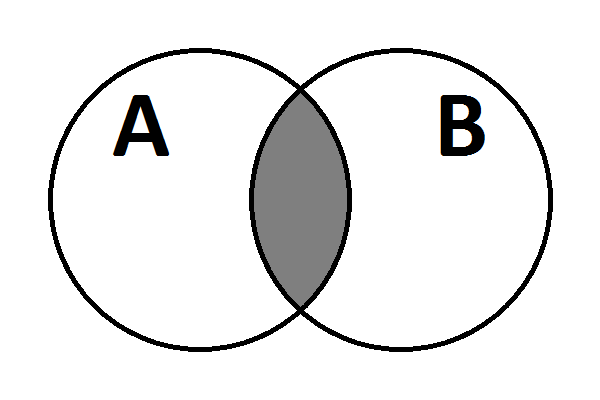
\includegraphics[scale=0.3]{../images/venn_diagram_a_intersects_b}
    \caption{The intersection between two sets makes math a bit tricky}
    \label{fig:venn_a_inter_b}
  \end{center}
\end{figure}

\begin{description}
  \item[1.] $P(A \cup B) = P(A) + P(B) - P(A \cap B) = P(A \setminus B) + P(A \cap B) + P(B \setminus A)$
            \\ The probability that one of two events happens is their individual probabilities minus the probability that both events happen simultaneously (otherwise we would account for that case twice, see also figure \nolinebreak\ref{fig:venn_a_inter_b}).
  \item[2.] $P(A \cup \neg A) = P(\Omega) = 1 = P(A) + P(\neg A)$
            \\ The probability that an event happens or not is 1.
  \item[3.] $P(A) = 1 - P(\neg A)$
            \\ The probability of an event to not happen is 1 minus the probability of the event (and vice versa).
\end{description}

\subsection{Random Variables \& Joint Distribution}
\index{Joint Distribution}\index{Random Variable}
An example for a joint distribution: You roll two dice, one is six-sided and red, the other one is four-sided and blue.
\begin{align*}
\mbox{R: }\Omega_R = \{1, ..., 6\} & & P(R=\omega) = \frac{1}{6}\ \forall\ \omega \in \Omega_R\\
\mbox{B: }\Omega_B = \{1, ..., 4\} & & P(B=\omega) = \frac{1}{4}\ \forall\ \omega \in \Omega_B
\end{align*}
The joint sample space $\Omega$ is $\Omega = \Omega_R \times \Omega_B$.

Since R and B are independent the joint probability\index{Joint Probability} is $ P(R, B) = \frac{1}{24}$ for each value of R, B.

More formally speaking it holds that $P(R=i, B=j) = \frac{1}{24}$ for all values of $i, j$ since $P(R, B) = P(R) \cdot P(B)$ for all independent $R, B$.



\subsection{Marginal and Conditional Probability}
For the following examples please refer to table \ref{tab:2014-04-25_cards} (page \pageref{tab:2014-04-25_cards}).

\subsubsection*{Marginal Probability}
The \textbf{Marginal Probability}\index{Marginal Probability} for $P(R=j)$ is:
\begin{align*}
P(R=j) = 
\begin{cases} 
\frac{5}{25} & \mbox{if } j = 1 \\ 
\frac{4}{25} & \mbox{else}
\end{cases}
\end{align*}

This can be calculated by summing up one dimension of the table.
\begin{align*}
P(R=j) = \sum\limits_{i \in \Omega_B} P(R=j, B=i)
\end{align*}

This can be written a bit more casual (here for B now):
\begin{align*}
P(B) = \sum\limits_R P(R, B) = 
\begin{cases} 
\frac{7}{25} & \mbox{if } B = 1 \\ 
\frac{6}{25} & \mbox{else}
\end{cases}
\end{align*}

\subsubsection*{Conditional Probability}
\index{Conditional Probability}In case a card was picked and we already know what number the red side shows,
$P(R, B) \neq P(R) \cdot P(B)$ is \textit{not independent}\index{Independence}. $P(R,B)$ is now dependent\index{Dependence} on the already known red number.

The probabilities that follow are:
\begin{align*}
P(B|R=1) =
\begin{cases} 
\frac{2}{5} & \mbox{if } B = 1 \\ 
\frac{1}{5} & \mbox{else}
\end{cases}\\
P(B|R=2, ..., 6) = \frac{1}{4}
\end{align*}

The conditional probability $P(A|B)$ (read: $P$ of $A$ given $B$) can be expressed as follows:
\begin{align*}
P(A|B)         &= \frac{P(A, B)}{\sum\limits_A P(A, B)} = \frac{P(A, B)}{P(B)} \\
\mbox{where}   & \\
P(A, B)        &\mbox{ is the joint pobability} \\
\sum\limits_A P(A, B) &\mbox{ is the marginal probability} \\
P(A, B)        &\mbox{ is a function of A (because B is fixed)}\\
P(B)           &\mbox{ is the renorm}
\end{align*}

With the product rule\index{Product Rule} $P(A|B)P(B) = P(A, B) = P(B|A)P(A)$ we can derive \textbf{Bayes' rule}\index{Bayes' Rule}:
\begin{align*}
P(B|A) &= \frac{P(A|B)P(B)}{P(A)} = \frac{P(A|B)P(B)}{\sum\limits_B P(A|B)P(B)} \\
\mbox{where we call}   & \\
P(B|A)  &\mbox{ posterior} \\
P(A|B)  &\mbox{ likelihood} \\
P(B)    &\mbox{ prior} \\
P(A)    &\mbox{ evidence}
\end{align*}

\end{document}